% =========================================================================== %
% TeX input file: "Run the Final Application"
%
% WARNING: this tex file does not compile standalone, it needs to be embedded
% in a master tex document (e.g. Introduction.tex)
% =========================================================================== %


We are now ready to run the completed ''Hello World!'' application by first starting the server and then the clients. 
This results in running clients as shown in \figref{helloworld_finished}. 
The mobile version of the client can be started from the Scout SDK by clicking on the \link{Smartphone Devices} in the product launchers section. 
Alternatively, manually change the applications URL from \java{http://localhost:8082/web} to \java{http://localhost:8082/mobile}. 

\begin{figure}
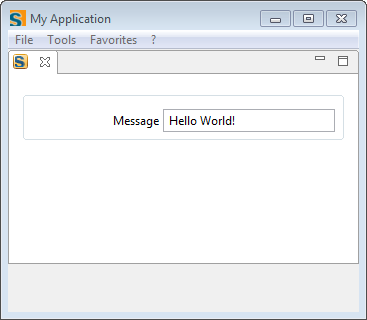
\includegraphics[width=4.5cm]{helloworld_swt.png} \hspace{3mm}
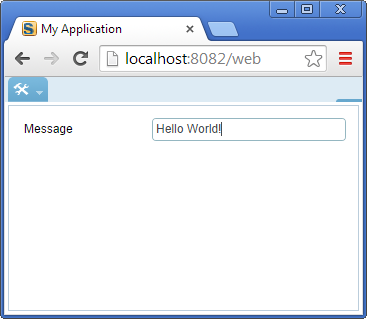
\includegraphics[width=4.5cm]{helloworld_web.png} \hspace{3mm}
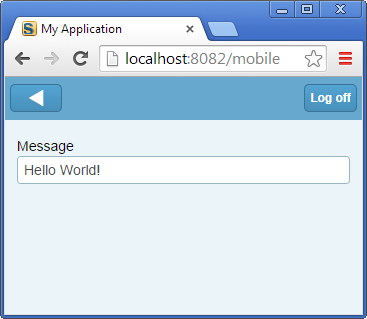
\includegraphics[width=4.5cm]{helloworld_mobile.png}
\caption{Running the complete ''Hello World!'' application with an SWT client, as a web application and a mobile application.}
\figlabel{helloworld_finished}
\end{figure}

Congratulations, you just have implemented your first Scout client server application!

% =========================================================================== %
% EOF TeX input file
% =========================================================================== %
